% =====================================================================
% Cuarta parte – Estimación del software
% =====================================================================
\section{Supuestos comunes}

Para comparar los modelos usamos los mismos supuestos. Todos los cálculos se reproducen con \codigo{docs/scripts/estimacion.py} (Apéndice \ref{ap:estimacion}).

\begin{itemize}
  \item Una persona-mes (PM) equivale a 160 horas.
  \item Cuando el modelo no da el tiempo de desarrollo, se calcula con la ecuación de calendario de COCOMO, $T = 2{,}5 \cdot E^{0{,}38}$ meses, y el número de personas con $P = E/T$ \parencite{boehm2000}.
  \item El costo de una persona-mes sale de una tarifa justificada (sección \ref{sec:presupuesto}): \$6\,646\,961.
\end{itemize}

\section{Puntos de función}

Conteo IFPUG \parencite{albrecht1979,ifpug2010} sobre el sistema completo.

\begin{table}[H]
\caption{Conteo de puntos de función no ajustados}
\label{tab:pf}
\footnotesize
\begin{tabularx}{\linewidth}{L{1cm} Y L{1.4cm} L{0.8cm} L{0.8cm}}
\toprule
Tipo & Elementos identificados & Complejidad & Peso & PF \\
\midrule
ILF & users, category, budget, transactions, saving\_goal (5) & Baja & 7 & 35 \\
EIF & Google userinfo (1) & Baja & 5 & 5 \\
EI & Crear y actualizar transacción, presupuesto y meta (6) & Media & 4 & 24 \\
EI & Registro, login, Google, perfil, contraseña, moneda, subir y eliminar foto, eliminar cuenta, eliminar transacción, CRUD de categoría (3), eliminar presupuesto, eliminar meta, marcar día (16) & Baja & 3 & 48 \\
EO & Presupuestos con gasto y porcentaje, progreso de metas, resumen, recurrentes automáticas (4) & Media & 5 & 20 \\
EO & Gráficas de torta, barras y áreas (1) & Alta & 7 & 7 \\
EQ & Historial, categorías, \codigo{/users/me}, detalle de meta (4) & Baja & 3 & 12 \\
\midrule
\multicolumn{4}{l}{Puntos de función no ajustados (PFNA)} & 151 \\
\bottomrule
\end{tabularx}
\tablenote{Fuente: elaboración propia.}
\end{table}

\begin{table}[H]
\caption{Características generales del sistema}
\label{tab:gsc}
\footnotesize
\begin{tabularx}{\linewidth}{Y L{1cm} Y L{1cm}}
\toprule
Característica & Valor & Característica & Valor \\
\midrule
Comunicación de datos & 4 & Actualización en línea & 4 \\
Procesamiento distribuido & 3 & Procesamiento complejo & 2 \\
Rendimiento & 2 & Reutilización & 2 \\
Configuración muy utilizada & 2 & Facilidad de instalación & 2 \\
Tasa de transacciones & 2 & Facilidad de operación & 3 \\
Entrada de datos en línea & 5 & Múltiples sitios & 3 \\
Eficiencia del usuario final & 4 & Facilidad de cambio & 3 \\
\midrule
\multicolumn{3}{l}{Total (TDI)} & 41 \\
\bottomrule
\end{tabularx}
\tablenote{Fuente: elaboración propia.}
\end{table}

\begin{align*}
VAF &= 0{,}65 + 0{,}01 \times 41 = 1{,}06 & PF &= 151 \times 1{,}06 = 160{,}06\\
E &= 160{,}06 \times 8\ \text{h/PF} = 1\,280\ \text{h} = 8{,}00\ \text{PM} & T &= 2{,}5 \times 8{,}00^{0{,}38} = 5{,}51\ \text{meses}\\
& & P &= 8{,}00 / 5{,}51 = 1{,}45
\end{align*}

La productividad de 8 horas por punto de función es un supuesto típico para desarrollo web con lenguajes de alto nivel.

\section{Puntos de función COSMIC}

El método COSMIC (ISO/IEC 19761) mide el tamaño funcional contando los \textbf{movimientos de datos} de cada proceso funcional: entradas (E) y salidas (X) que cruzan la frontera con un usuario funcional, y lecturas (R) y escrituras (W) en el almacenamiento persistente. Cada movimiento vale 1 CFP (\emph{COSMIC Function Point}). Los usuarios funcionales son el usuario de la aplicación, el servicio de Google y el reloj del programador de tareas; los grupos de datos son usuario, categoría, presupuesto, transacción y meta. Contamos un movimiento por grupo de datos y una salida para los mensajes de confirmación o error de cada proceso.

\begin{table}[H]
\caption{Conteo COSMIC por proceso funcional}
\label{tab:cosmic}
\scriptsize
\setlength{\tabcolsep}{3pt}
\begin{tabularx}{\linewidth}{Y *{5}{c} | Y *{5}{c}}
\toprule
Proceso & E & X & R & W & CFP & Proceso & E & X & R & W & CFP \\
\midrule
Registrar usuario & 1 & 1 & 1 & 1 & 4 & Iniciar sesión & 1 & 2 & 1 & 0 & 4 \\
Iniciar sesión con Google & 2 & 3 & 1 & 1 & 7 & Consultar perfil & 1 & 1 & 1 & 0 & 3 \\
Editar perfil & 1 & 1 & 1 & 1 & 4 & Cambiar contraseña & 1 & 1 & 1 & 1 & 4 \\
Cambiar moneda & 1 & 1 & 1 & 1 & 4 & Subir foto de perfil & 1 & 1 & 1 & 1 & 4 \\
Eliminar foto de perfil & 1 & 1 & 1 & 1 & 4 & Eliminar cuenta y sus datos & 1 & 1 & 1 & 5 & 8 \\
Listar categorías & 1 & 1 & 1 & 0 & 3 & Crear categoría & 1 & 1 & 1 & 1 & 4 \\
Editar categoría & 1 & 1 & 1 & 1 & 4 & Eliminar categoría & 1 & 1 & 2 & 2 & 6 \\
Registrar transacción & 1 & 1 & 1 & 1 & 4 & Consultar historial con filtros & 1 & 1 & 2 & 0 & 4 \\
Editar transacción & 1 & 1 & 2 & 1 & 5 & Eliminar transacción & 1 & 1 & 1 & 1 & 4 \\
Crear presupuesto & 1 & 1 & 1 & 1 & 4 & Consultar presupuestos con gasto & 1 & 1 & 3 & 0 & 5 \\
Editar presupuesto & 1 & 1 & 2 & 1 & 5 & Eliminar presupuesto & 1 & 1 & 1 & 1 & 4 \\
Crear meta con plan diario & 1 & 1 & 1 & 1 & 4 & Consultar metas y progreso & 1 & 1 & 1 & 0 & 3 \\
Editar meta & 1 & 1 & 2 & 1 & 5 & Eliminar meta & 1 & 1 & 1 & 1 & 4 \\
Marcar o desmarcar día & 1 & 1 & 1 & 1 & 4 & Ver resumen del mes & 1 & 1 & 2 & 0 & 4 \\
Ver gráficas & 1 & 1 & 2 & 0 & 4 & Generar recurrentes (reloj) & 1 & 0 & 1 & 1 & 3 \\
\midrule
\multicolumn{6}{l|}{Totales: E = 31, X = 32, R = 39, W = 27} & \multicolumn{6}{l}{\textbf{Tamaño: 129 CFP}} \\
\bottomrule
\end{tabularx}
\vspace{6pt}
\tablenote{Los 30 procesos cubren los 20 RF. «Eliminar cuenta» escribe en los cinco grupos de datos por la eliminación en cascada (D-11); «Eliminar categoría» lee las transacciones para impedir el borrado (D-05). Fuente: elaboración propia.}
\end{table}

Para que la comparación con IFPUG dependa solo del tamaño, usamos la misma productividad supuesta, 8 horas por unidad:
\[
E = \frac{129 \times 8}{160} = 6{,}45\ \text{PM} \qquad T = 2{,}5 \times 6{,}45^{0{,}38} = 5{,}08\ \text{meses} \qquad P = \frac{6{,}45}{5{,}08} = 1{,}27
\]
con un costo de talento humano de $6{,}45 \times \$6\,646\,961 = \$42\,872\,896$. COSMIC da un tamaño menor que IFPUG (129 frente a 160 unidades) porque no pondera la complejidad de cada función ni aplica el factor de ajuste: cuenta solo movimientos de datos.

\section{Puntos de casos de uso}

Método de \textcite{karner1993} sobre los 14 casos de uso de la Figura \ref{fig:cu-general}.

\begin{table}[H]
\caption{Peso de los actores y de los casos de uso}
\label{tab:pcu}
\footnotesize
\begin{tabularx}{\linewidth}{L{2.6cm} Y L{0.8cm} L{0.9cm}}
\toprule
Elemento & Detalle & Peso & Total \\
\midrule
Actor complejo & Usuario (interfaz gráfica) & 3 & 3 \\
Actor medio & Google OAuth (protocolo HTTP) & 2 & 2 \\
Actor simple & Programador de tareas (API interna) & 1 & 1 \\
\multicolumn{3}{l}{UAW} & 6 \\
\midrule
CU simples (3) & CU04 Registrarse, CU05 Iniciar sesión, CU08 Editar o eliminar transacción & 5 & 15 \\
CU medios (9) & CU01, CU06, CU07, CU09, CU10, CU11, CU12, CU13, CU14 & 10 & 90 \\
CU complejos (2) & CU02 Gestionar presupuesto, CU03 Gestionar meta & 15 & 30 \\
\multicolumn{3}{l}{UUCW} & 135 \\
\bottomrule
\end{tabularx}
\tablenote{Fuente: elaboración propia.}
\end{table}

Los factores técnicos T1 a T13 valen 3, 3, 3, 2, 1, 1, 3, 3, 4, 2, 1, 0 y 1, que con sus pesos dan $TF = 31$. Los factores de entorno E1 a E8 valen 3, 2, 3, 4, 4, 3, 1 y 1, que dan $EF = 18{,}5$.
\begin{align*}
UUCP &= 6 + 135 = 141 & TCF &= 0{,}6 + 0{,}01 \times 31 = 0{,}91\\
ECF &= 1{,}4 - 0{,}03 \times 18{,}5 = 0{,}845 & UCP &= 141 \times 0{,}91 \times 0{,}845 = 108{,}42\\
E &= 108{,}42 \times 20\ \text{h} = 13{,}55\ \text{PM} & T &= 6{,}73\ \text{meses};\ P = 2{,}01
\end{align*}

\section{Puntos de objeto}

Modelo de composición de aplicaciones de COCOMO II \parencite{boehm2000}.

\begin{table}[H]
\caption{Conteo de puntos de objeto}
\label{tab:po}
\footnotesize
\begin{tabularx}{\linewidth}{L{3.2cm} Y L{0.8cm} L{0.9cm}}
\toprule
Tipo & Objetos & Peso & Total \\
\midrule
Pantallas simples (4) & Home, CategoriaFormModal, ConfirmarEliminar, ConfirmarEliminarCategoria & 1 & 4 \\
Pantallas medias (7) & AuthPage, Historial, Categorías, Configuración, ModalTransaccion, DetalleTransaccion, MetaFormModal & 2 & 14 \\
Pantallas difíciles (5) & Resumen, Gráficas, Presupuestos, Metas (reto), PresupuestoModal & 3 & 15 \\
Componentes 3GL (8) & Módulos de rutas y autenticación del backend, programador & 10 & 80 \\
\midrule
\multicolumn{3}{l}{Puntos de objeto (PO)} & 113 \\
\bottomrule
\end{tabularx}
\tablenote{Fuente: elaboración propia.}
\end{table}

\[
NOP = 113 \times (1 - 0{,}20) = 90{,}4 \qquad E = \frac{90{,}4}{13} = 6{,}95\ \text{PM} \qquad T = 5{,}22\ \text{meses};\ P = 1{,}33
\]
con 20\,\% de reúso (React, Recharts y FastAPI) y productividad nominal de 13 NOP por persona-mes.

\section{Puntos de historia}

Las historias de usuario corresponden a los requisitos funcionales y se estimaron con la serie de Fibonacci \parencite{cohn2005}.

\begin{table}[H]
\caption{Historias de usuario y puntos de historia}
\label{tab:ph}
\footnotesize
\begin{tabularx}{\linewidth}{L{1.1cm} Y L{1.6cm} L{0.8cm}}
\toprule
ID & Como usuario, quiero\ldots & RF & PH \\
\midrule
HU01 & registrarme e iniciar sesión (también con Google) & RF01, RF02 & 5 \\
HU02 & registrar un ingreso o un gasto & RF03 & 5 \\
HU03 & programar transacciones recurrentes & RF04, RF05 & 8 \\
HU04 & editar y eliminar transacciones & RF06 & 3 \\
HU05 & consultar el historial con filtros & RF07 & 5 \\
HU06 & ver el resumen financiero del mes & RF08 & 5 \\
HU07 & ver gráficas de mis movimientos & RF09 & 8 \\
HU08 & gestionar categorías propias & RF10 & 5 \\
HU09 & crear presupuestos con 4 tipos de período & RF11, RF13 & 13 \\
HU10 & ver el gasto ejecutado y las alertas & RF12, RF14 & 8 \\
HU11 & crear metas con un plan de ahorro diario & RF15, RF16, RF18 & 13 \\
HU12 & marcar los días del reto y ver el progreso & RF17 & 5 \\
HU13 & configurar el perfil, la moneda y la foto & RF19 & 3 \\
HU14 & cambiar el tema claro u oscuro & RF20 & 2 \\
HU15 & ver una página informativa pública & — & 1 \\
\midrule
\multicolumn{3}{l}{Total} & 89 \\
\bottomrule
\end{tabularx}
\tablenote{Fuente: elaboración propia.}
\end{table}

Con una velocidad supuesta de 20 puntos por sprint de 2 semanas: $89/20 = 4{,}45$ sprints, es decir, 8,9 semanas o $T = 2{,}05$ meses; con los 3 desarrolladores, $E = 2{,}05 \times 3 = 6{,}16$ PM. En la entrega anterior se supusieron 2 personas; el equipo real tuvo 3.

\section{Estimación con herramienta: COCOMO II}

Se usó la calculadora en línea de COCOMO II (modelo post-arquitectura, COCOMO II.2000) de Ray Madachy \parencite{boehm2000} y se verificó con el script. La entrada es el tamaño de la lógica del producto como se desarrolló (Python, JavaScript y JSX del commit \codigo{0efe28b}): 6\,228 SLOC según la medición de la Tercera parte (la entrega anterior usó 6\,154 con la versión previa del script).

\begin{align*}
E_{esc} &= 0{,}91 + 0{,}01 \textstyle\sum SF = 0{,}91 + 0{,}01 \times 18{,}97 = 1{,}0997 \quad \text{(factores de escala nominales)}\\
EAF &= \textstyle\prod EM = 0{,}866\\
&\quad (\text{DOCU } 0{,}91;\ \text{PVOL } 0{,}87;\ \text{APEX } 1{,}10;\ \text{PLEX } 1{,}09;\ \text{LTEX } 1{,}09;\ \text{TOOL } 0{,}90;\ \text{SITE } 0{,}93)\\
PM &= 2{,}94 \times 6{,}228^{1{,}0997} \times 0{,}866 = 19{,}03\\
T_{DEV} &= 3{,}67 \times 19{,}03^{0{,}28 + 0{,}2(1{,}0997 - 0{,}91)} = 9{,}36\ \text{meses};\quad P = 19{,}03 / 9{,}36 = 2{,}03
\end{align*}

\begin{figure}[H]
\centering
\caption{Calculadora COCOMO II con la entrada de 6\,154 SLOC de la entrega anterior: 18,8 PM y 9,3 meses}
\label{fig:cocomo}
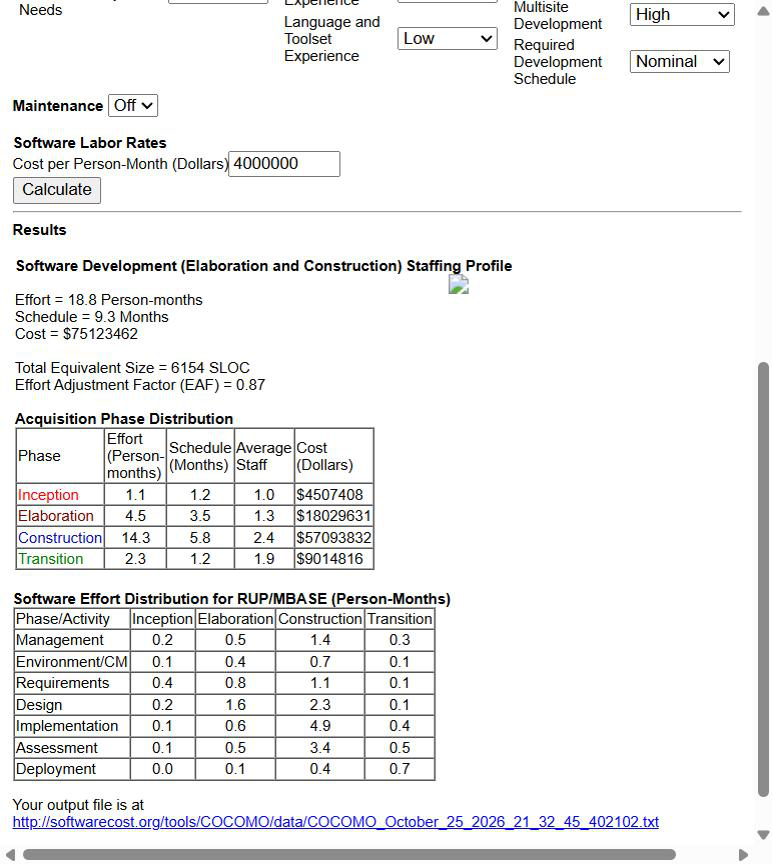
\includegraphics[width=0.75\linewidth, height=0.35\textheight, keepaspectratio]{previo/cocomo_calculadora.png}
\figurenote{Con 6\,228 SLOC el script da 19,03 PM y 9,36 meses (Figura \ref{fig:estimacion-script}). Fuente: elaboración propia.}
\end{figure}

\begin{figure}[H]
\centering
\caption{Recálculo de los seis modelos paramétricos y del presupuesto con \codigo{estimacion.py}}
\label{fig:estimacion-script}
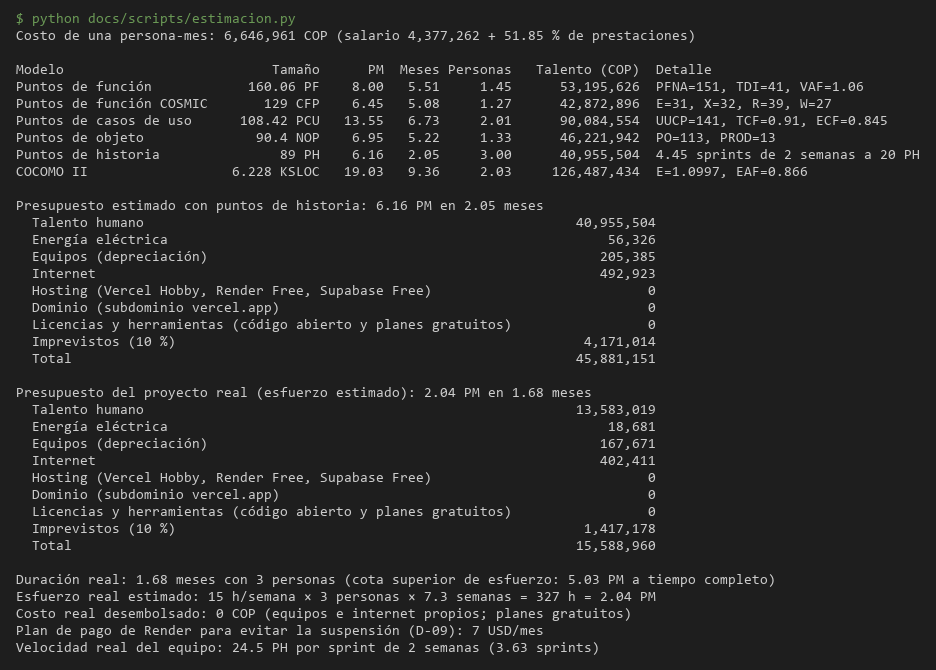
\includegraphics[width=\linewidth]{../evidencias/estimacion_salida.png}
\figurenote{Fuente: elaboración propia.}
\end{figure}

\section{Estimación con una herramienta de inteligencia artificial}

Usamos el asistente \textbf{Claude Opus 5.5} (Anthropic) el 26 de noviembre de 2026. Le dimos la descripción del proyecto y le pedimos una estimación de esfuerzo, tiempo y personas, sin mostrarle los resultados de los otros modelos.

\paragraph{Instrucción (prompt).} «Estima el esfuerzo en personas-mes, la duración en meses y el número de personas para desarrollar esta aplicación web: frontend en React 19 con Vite y backend en FastAPI con SQLAlchemy y PostgreSQL; 20 requisitos funcionales (registro e inicio de sesión con correo y Google, transacciones con recurrencia, historial con filtros, resumen y gráficas, categorías propias, presupuestos con cuatro tipos de período y alertas, metas de ahorro con plan diario y días marcables, perfil, moneda y tema); 5 tablas; despliegue en Vercel, Render y Supabase; pruebas unitarias, de integración y de aceptación. Equipo de 3 estudiantes. Explica cómo llegas al resultado.»

\paragraph{Respuesta resumida.} El asistente estimó por descomposición de tareas (ascendente), en horas de un desarrollador junior:

\begin{table}[H]
\caption{Estimación de la herramienta de IA por módulo}
\label{tab:ia}
\footnotesize
\begin{tabularx}{\linewidth}{Y r}
\toprule
Módulo & Horas \\
\midrule
Autenticación (correo, Google, JWT) & 80 \\
Transacciones, recurrencia e historial con filtros & 140 \\
Categorías propias & 40 \\
Presupuestos con períodos y alertas & 130 \\
Metas de ahorro con plan diario & 120 \\
Resumen y gráficas & 100 \\
Perfil, moneda, foto y tema & 60 \\
Despliegue y configuración & 50 \\
Pruebas & 160 \\
\midrule
\textbf{Total} & \textbf{880 h = 5,5 PM} \\
\bottomrule
\end{tabularx}
\tablenote{Fuente: respuesta de Claude Opus 5.5, organizada por el equipo.}
\end{table}

Propuso una duración de \textbf{2,5 meses}, con $P = 5{,}5 / 2{,}5 = 2{,}2$ personas a tiempo completo, y un costo de talento humano de $5{,}5 \times \$6\,646\,961 = \$36\,558\,284$. La herramienta advirtió que su estimación depende de la experiencia del equipo y que debe calibrarse con datos propios, igual que los modelos paramétricos.

\section{Presupuesto}\label{sec:presupuesto}

\paragraph{Tarifa del talento humano.} Tomamos como salario de un desarrollador junior 2,5 salarios mínimos: según el Observatorio Laboral para la Educación, el 65,6\,\% de los graduados de programas TIC (programación, sistemas, desarrollo de software) gana más de 2,5 salarios mínimos en su primer empleo \parencite{barona2026}. Con el salario mínimo de 2026, \$1\,750\,905 \parencite{decreto1470}, el salario es de \$4\,377\,262. A ese valor sumamos la carga prestacional de ley: cesantías (8,33\,\%), intereses sobre cesantías (1\,\%), prima (8,33\,\%), vacaciones (4,17\,\%), pensión (12\,\%), salud (8,5\,\%), ARL de riesgo I (0,522\,\%), caja de compensación (4\,\%), ICBF (3\,\%) y SENA (2\,\%), en total 51,85\,\%. El costo de una persona-mes es \textbf{\$6\,646\,961}. Una empresa exonerada de los aportes de salud, ICBF y SENA pagaría menos; usamos el caso completo como cota superior.

\paragraph{Esfuerzo real estimado.} El equipo no registró horas. Como estudiantes que cursaban otras asignaturas, estimamos una dedicación de 15 horas por semana por persona: $15 \times 3 \times 7{,}3\ \text{semanas} = 327$ horas, es decir, \textbf{2,04 PM} en los 1,68 meses del desarrollo.

\paragraph{Costo real y valor estimado.} El equipo no desembolsó dinero: usó sus propios computadores e internet, y planes gratuitos de hosting y herramientas. El \textbf{costo real desembolsado fue \$0}. La Tabla \ref{tab:presupuesto} estima cuánto costaría el proyecto si se contratara: la primera columna usa la estimación por puntos de historia y la segunda, el esfuerzo real estimado.

\begin{table}[H]
\caption{Presupuesto desglosado: estimación y proyecto real}
\label{tab:presupuesto}
\footnotesize
\begin{tabularx}{\linewidth}{L{2.4cm} Y L{2.1cm} L{2.1cm}}
\toprule
Rubro & Cálculo y fuente & Estimado (6,16 PM; 2,05 meses) & Real (2,04 PM; 1,68 meses) \\
\midrule
Talento humano & PM × \$6\,646\,961 & 40\,955\,504 & 13\,583\,019 \\
Equipos & Depreciación de 3 portátiles de \$2\,000\,000 \parencite{portafolio_portatiles} a 60 meses (20\,\% anual, \cite{estatuto137}) & 205\,385 & 167\,671 \\
Energía eléctrica & Horas × 65 W × \$879/kWh (costo promedio en la zona de Afinia, \cite{rtvc2026}) & 56\,326 & 18\,681 \\
Internet & 3 planes de fibra de \$80\,000 al mes \parencite{cuantomecuesta2026} durante el proyecto & 492\,923 & 402\,411 \\
Hosting & Vercel Hobby, Render Free y Supabase Free \parencite{vercel2026,render2026,supabase2026} & 0 & 0 \\
Dominio & Subdominio \codigo{vercel.app} & 0 & 0 \\
Licencias y herramientas & Código abierto (React, FastAPI, pytest, Cypress, JMeter, ZAP, SonarQube Community) y planes gratuitos (LambdaTest) & 0 & 0 \\
\midrule
Subtotal & & 41\,710\,138 & 14\,171\,782 \\
Imprevistos & 10\,\% del subtotal & 4\,171\,014 & 1\,417\,178 \\
\midrule
\textbf{Total} & & \textbf{45\,881\,151} & \textbf{15\,588\,960} \\
\bottomrule
\end{tabularx}
\tablenote{Son valores estimados: el precio del portátil, el consumo de 65 W, el plan de internet completo (cota superior, porque el hogar también lo usa para otras cosas) y las 15 horas semanales son supuestos declarados. Fuente: elaboración propia con \codigo{estimacion.py}.}
\end{table}

\paragraph{Costeo por servicios.} Una empresa también puede cotizar por servicio o por unidad funcional en lugar de por horas. Con el costo real estimado (\$15\,588\,960) y el tamaño medido, cada punto de función IFPUG cuesta $15\,588\,960 / 160{,}06 = \$97\,395$ y cada CFP, $15\,588\,960 / 129 = \$120\,845$. Repartido en proporción a los puntos de historia (Tabla \ref{tab:ph}), el servicio de presupuestos (HU09 y HU10, 21 de 89 puntos) costaría \$3\,678\,294; el de metas de ahorro (HU11 y HU12, 18 puntos), \$3\,152\,823; y el de transacciones (HU02 a HU05, 21 puntos), \$3\,678\,294. Esta forma de cotizar permite presupuestar mejoras futuras por separado.

\paragraph{Riesgo de costo.} El hosting cuesta \$0 porque se usan planes gratuitos, y es la causa del defecto D-09 (la API se suspende tras la inactividad). Mantener la API siempre disponible exige el plan Starter de Render, de USD 7 al mes \parencite{render2026}; la base de datos seguiría en Supabase sin costo.

\section{Análisis comparativo}

\begin{table}[H]
\caption{Comparación de los modelos de estimación con el proyecto real}
\label{tab:comparacion-estimacion}
\footnotesize
\begin{tabularx}{\linewidth}{L{3cm} L{2.1cm} *{4}{>{\raggedleft\arraybackslash}X}}
\toprule
Modelo & Tamaño & Esfuerzo (PM) & Tiempo (meses) & Personas & Talento (COP) \\
\midrule
Puntos de función (IFPUG) & 160,06 PF & 8,00 & 5,51 & 1,45 & 53\,195\,626 \\
Puntos de función COSMIC & 129 CFP & 6,45 & 5,08 & 1,27 & 42\,872\,896 \\
Puntos de casos de uso & 108,42 PCU & 13,55 & 6,73 & 2,01 & 90\,084\,554 \\
Puntos de objeto & 90,4 NOP & 6,95 & 5,22 & 1,33 & 46\,221\,942 \\
Puntos de historia & 89 PH & 6,16 & 2,05 & 3,00 & 40\,955\,504 \\
COCOMO II & 6,228 KSLOC & 19,03 & 9,36 & 2,03 & 126\,487\,434 \\
Herramienta de IA & 880 h & 5,50 & 2,50 & 2,20 & 36\,558\,284 \\
\midrule
\textbf{Real (estimado)} & — & \textbf{2,04} & \textbf{1,68} & \textbf{3} & \textbf{13\,583\,019} \\
\bottomrule
\end{tabularx}
\tablenote{El esfuerzo real se estimó con 15 horas por semana por persona durante los 51 días de desarrollo (21 de abril a 10 de junio de 2026); a tiempo completo, la cota superior sería 5,03 PM. El costo real desembolsado fue \$0. Fuente: elaboración propia.}
\end{table}

\begin{figure}[H]
\centering
\caption{Tiempo estimado por modelo frente a la duración real}
\label{fig:estimacion-barras}
\begin{tikzpicture}[x=0.9cm, y=0.8cm, font=\footnotesize]
\foreach \m/\v/\y in {Puntos de función/5.51/7, COSMIC/5.08/6, Casos de uso/6.73/5, Puntos de objeto/5.22/4, Puntos de historia/2.05/3, Herramienta de IA/2.50/2, COCOMO II/9.36/1} {
  \node[anchor=east] at (-0.1,\y) {\m};
  \fill[gris] (0,\y-0.3) rectangle (\v,\y+0.3);
  \node[anchor=west] at (\v+0.1,\y) {\v};
}
\draw[acento, very thick, dashed] (1.68,0.4) -- (1.68,7.6);
\node[acento, anchor=south] at (1.68,7.6) {Real: 1,68 meses};
\draw[flecha] (0,0.4) -- (10.2,0.4) node[right]{meses};
\foreach \x in {0,2,4,6,8,10} \node[below] at (\x,0.4) {\x};
\end{tikzpicture}
\figurenote{Fuente: elaboración propia.}
\end{figure}

\paragraph{Coherencia con el cronograma real.} El desarrollo del producto duró 1,68 meses con 3 personas (Figura \ref{fig:gantt}).
\begin{itemize}
  \item Los \textbf{puntos de historia} son los únicos coherentes con esa duración: estiman 2,05 meses, un 22\,\% más que lo real. En esfuerzo, todos los modelos superan los 2,04 PM estimados, porque suponen dedicación de tiempo completo. Con la duración real, el equipo tuvo una velocidad de 24,5 puntos por sprint de 2 semanas, mayor que los 20 supuestos; con esa velocidad calibrada, el modelo reproduce la duración real.
  \item La \textbf{herramienta de IA} es la segunda más cercana: 2,5 meses, un 49\,\% más que lo real. Al estimar por módulos, como un equipo, llega a un esfuerzo parecido al de los puntos de historia (5,5 frente a 6,16 PM).
  \item \textbf{Puntos de función} (IFPUG y COSMIC) y \textbf{puntos de objeto} coinciden entre sí (6,5 a 8 PM, unos 5 meses), pero triplican la duración real. Suponen un equipo de 1,3 a 1,5 personas a tiempo completo, mientras que el equipo real fue de 3 estudiantes que trabajaron en paralelo.
  \item \textbf{COCOMO II} y \textbf{puntos de casos de uso} sobrestiman más (13,6 a 19 PM y 6,7 a 9,4 meses) porque suponen un proceso industrial con documentación, gestión y pruebas formales. Parte de ese esfuerzo sí existió, pero después: la fase de calidad (pruebas, métricas y correcciones) se hizo entre agosto y noviembre de 2026 y no está en los 1,68 meses del desarrollo.
\end{itemize}

\paragraph{Modelo más viable.} Para planificar un proyecto académico ágil con un equipo pequeño, los \textbf{puntos de historia} son el modelo más viable: se basan en las historias que el equipo ya usaba en Scrum, se calibran con la velocidad real y fueron los que más se acercaron al cronograma. Para presupuestar una versión de producción, que debe incluir el esfuerzo de calidad, los \textbf{puntos de función} son la referencia más estable e independiente de la tecnología.

\section{Conclusiones de la estimación}

\begin{itemize}
  \item Las siete estimaciones ubican el proyecto entre 5,5 y 19 PM y entre 2 y 9,4 meses; la dispersión muestra que toda estimación debe declarar sus supuestos y calibrarse con datos del propio equipo.
  \item Los puntos de historia, recalculados con el equipo real de 3 personas, son los más cercanos a la duración real (2,05 frente a 1,68 meses). La velocidad real medida, 24,5 puntos por sprint, sirve para estimar proyectos futuros del mismo equipo.
  \item El equipo no gastó dinero (costo real desembolsado: \$0). Contratado a una tarifa justificada, el proyecto real habría costado unos \$15,6 millones y la estimación por puntos de historia da \$45,9 millones; en ambos casos el talento humano es más del 95\,\% del costo, porque la infraestructura usa planes gratuitos.
\end{itemize}
